%\documentclass[a1paper,landscape,showframe,fontscale=.42]{baposter}

%%THIS are the max size given by the COMPLENET website and is bigger than A1!:
%%\documentclass[paperwidth=42in, paperheight=42in,landscape,showframe,fontscale=.42]{baposter}
%%\documentclass[paperwidth=42in, paperheight=33.1in,landscape,showframe,fontscale=.42]{baposter}
\documentclass[a1paper,portrait,showframe,fontscale=.45]{baposter}

%%%%lualatex on
%\usepackage{luatextra}
\usepackage{fontspec}
%Ligatures={Contextual, Common, Historical, Rare, Discretionary}
\setmainfont[Mapping=tex-text]{Linux Libertine O}


\usepackage{enumerate}
\usepackage[english]{babel}
\usepackage{graphicx} %to insert pictures
\usepackage{color} %to set colors
\usepackage{algorithm,algorithmicx,algpseudocode}
\usepackage{mathtools}
\usepackage{latexsym}
\usepackage{caption}
\usepackage{multicol}
\usepackage{array}

\usepackage{float}
\usepackage{booktabs}
\algnewcommand\And{\textbf{and}}

\DeclarePairedDelimiter\abs{\lvert}{\rvert}%
\DeclarePairedDelimiter\norm{\lVert}{\rVert}%

\newcommand{\specialcell}[2][c]{%
	\begin{tabular}[#1]{@{}c@{}}#2\end{tabular}}


		\makeatletter
		\let\oldabs\abs
		\def\abs{\@ifstar{\oldabs}{\oldabs*}}
		\let\oldnorm\norm
		\def\norm{\@ifstar{\oldnorm}{\oldnorm*}}
		\makeatother


%\usepackage[top=1.5cm,bottom=2cm,left=2.5cm,right=2.5cm]{geometry}
%\linespread{1.5}\selectfont



		\author{Simon Carrignon}
		\definecolor{bordercol}{RGB}{255,255,255}

		\definecolor{headercol1}{RGB}{142,161,42}
		\definecolor{epnetcol}{RGB}{142,161,42}
		\definecolor{headercol2}{RGB}{255,255,255}
		\definecolor{headerfontcol}{RGB}{78,78,78}
		\definecolor{boxcolor}{RGB}{255,255,255}
		\definecolor{emphcol}{RGB}{106,105,180}

%%% Save space in lists. Use this after the opening of the list %%%%%%%%%%%%%%%%
		\newcommand{\compresslist}{
		\setlength{\itemsep}{1pt}
			\setlength{\parskip}{0pt}
			\setlength{\parsep}{0pt}
		}
		\newcommand{\coloremph}[1]{
			\textcolor{emphcol}{\bf#1}
		}


		\begin{document}

		\begin{poster}{
				borderColor=bordercol,
				headerColorOne=headercol1,
				headerColorTwo=headercol2,
				headerFontColor=headerfontcol,
	% Only simple background color used, no shading, so boxColorTwo isn't necessary
				boxColorOne=boxcolor,
				headershape=roundedright,
				headerfont=\Large\sf\bf,
				textborder=rectangle,
				headerborder=open,
				background=plain,
				bgColorOne=white,
				boxshade=plain,
				eyecatcher,
				columns=2
			}
			{
			}
			{
				Influence of the topology of cultural networks on the equilibrium of an exchange-based economy
			}
			{
				Ignacio Morer, 
				Simon Carrignon,
				and Xavier Rubio-Campillo\\
				{\small simon.carrignon@bsc.es}
			}
			{
				\setlength\fboxsep{0pt}
				\setlength\fboxrule{0.5pt}
				\begin{minipage}{14em}
			%\vspace*{\stretch{1}}
					
\includegraphics[height=8em]{logos/epnetLogo2.png}
			%\vspace*{\stretch{1}}
			%\includegraphics[angle=90,width=2.5em]{MemoireLophiss/images/logo_p7_large}
				\end{minipage}
			}

			\headerbox{Introduction}{name=introduction,column=0,row=0}{
				Cultural change comprises  processes that modify spread of information by social interaction within a population~\cite{boyd_origin_2005}  and numerous social scientists are using an evolutionary framework to model this~\cite{henrich_evolution_2003}.

				Here we use this framework to study the dynamics of an exchange based economy. This social activity depends on particular cultural traits: the value attributed to goods used to trade during the exchange. Multiple cultural processes could influence the way those values evolve through space and time leading to different dynamics.

				We focus on the way those values are transmitted and vary from individual to individual, and on the bias that affect this transmission. We propose a framework that allow us to implement and test hypotheses and claims made about the nature of such transmission processes and bias and study how those claims and hypotheses affects a given economy.

			}
			\headerbox{Model}{name=ud,column=1,row=0}{

				To explore the co-evolution between trade and cultural change we developed a framework where the different agents produce and trade goods. The model is composed of a population $Pop$ of $m$ agents. Each agent $i$ is defined by 2 vectors $Q^i$ and $V^i$ of size $n$. $Q^i$ stores the quantity of each good owned by $i$ and $V^i$ represents the price estimated by $i$ for each of the $n$ good.
%\begin{algorithm}[H]
%	\scriptsize
%\caption{Model}
%\label{algo:complete}
%	\begin{algorithmic}[1]
%	\State INITIALIZATION: 
%		\For{$i \in \#Pop$} \Comment{Initialize the agent with no goods and a random value vector}
%				\State $Q^i = (0, \cdots, 0)$
%				\State $V^i = (v^i_0, \cdots, v^i_n)$ \Comment{The values of $v^i_j$ are selected randomly}
%		\EndFor
%
%	\State SIMULATION:
%		\Loop{$~step \in TimeSteps$}
%			\For{$i \in Pop$}
%				\State $Production(Q^i)$
%			\EndFor
%			\For{$i \in Pop$}
%				\For{$j \in Pop$}
%					\State $TradeProcess(V^i,Q^i,V^j,Q^j)$
%				\EndFor		
%			\EndFor
%			\For{$i \in Pop$}
%				\State $ConsumeGoods(Q^i)$ \Comment{All goods are consumed}
%				\If{$ (step \mod CulturalStep) = 0$}	
%					\State $CulturalTransmission(V)$
%					\State $Innovation(V^i)$
%				\EndIf
%			\EndFor
%		\EndLoop
%\end{algorithmic}
%\end{algorithm}
				Given the prices attributed by the agents for each good ($V^i$), an exchange is made or not using the trade network (in green in the Figure~\ref{fig:feedbackSchema}). Given the quantities ($Q^i$) gathered, a score reflecting the ``economic success'' of each agent is attributed. Using this score, agents use here cultural network (in blue in the Figure~\ref{fig:feedbackSchema}) to update the value attributed to each good $V^i$.

				\begin{figure}[H]
					\centering
					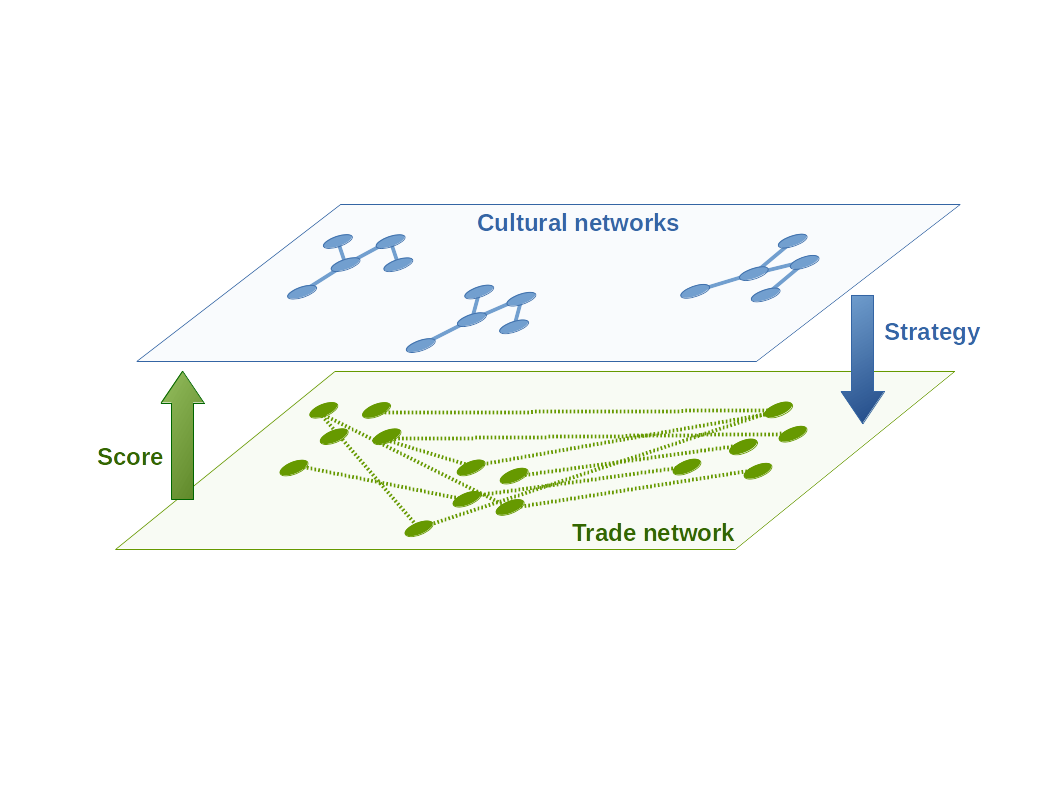
\includegraphics[trim={2cm 6cm 2cm 5cm},clip,width=10cm]{img/trade-cultural.png}
					\caption{ {\small Illustration of the interaction between the Trade network and the Cultural networks}}
					\label{fig:feedbackSchema}
				\end{figure}		


		%    We first compare the impact of different $CulturalTransmission$ mechanism on the distribution of frequencies of traits (the belief about the price of each goods). 
		%    \begin{figure}[H]
		%	\centering
		%	\setlength{\columnseprule}{0pt}
		%	\begin{multicols}{2}
		%	    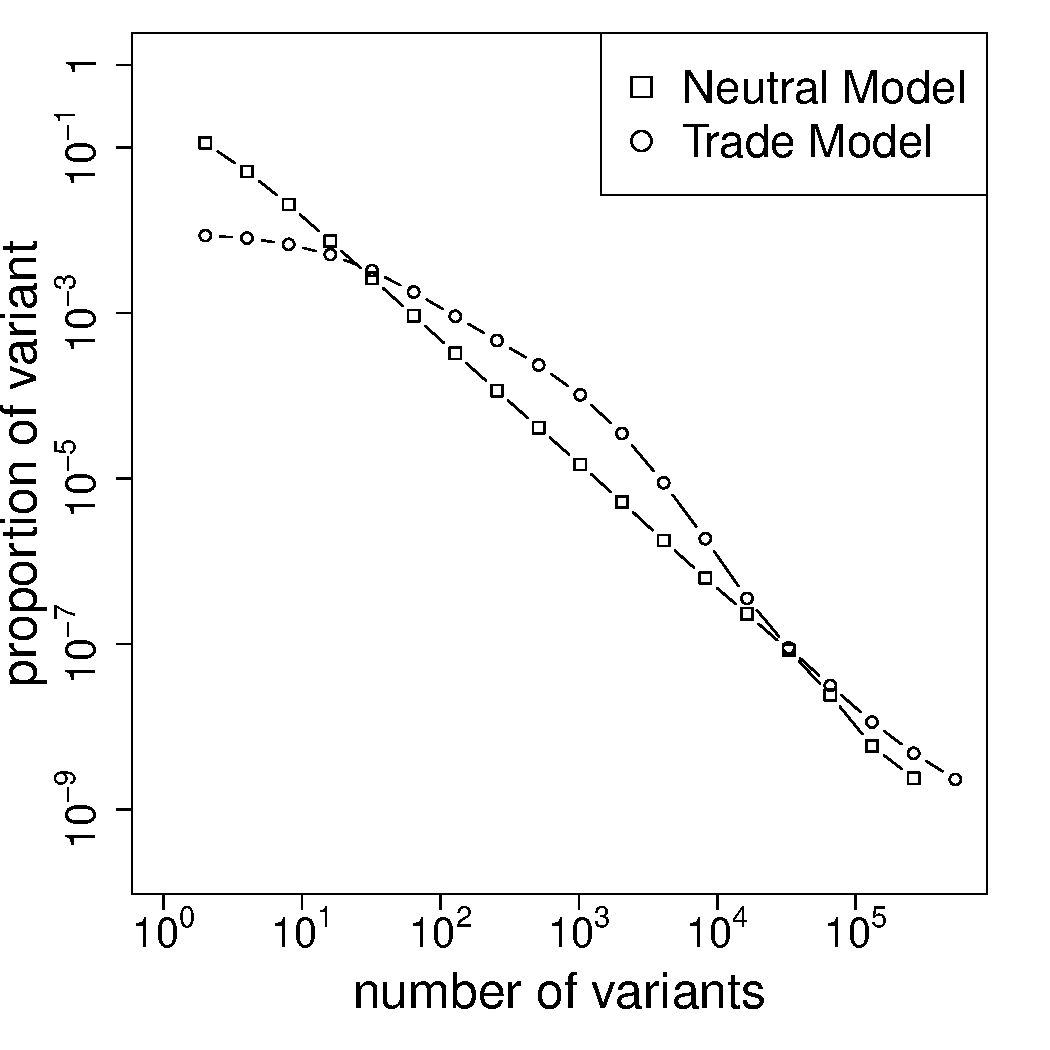
\includegraphics[width=5.2cm]{img/2SetupDistribA.pdf} 
		%	    \caption{Comparaison of the distribution of frequencies between the neutral and the trade model.}
		%	    \label{fig:2setDi}
		%	\end{multicols}
		%    \end{figure}
		%    \vspace{-.8cm}
		%    The figure~\ref{fig:2setDi} shows that when $CulturalTransmission$ is neutral (agents randomly copy prices) the distribution follow the well know power law \cite{bentley_random_2004} but when transmission is not neutral but biased by the economical success of the agents, the power law disappear.

			}




			\headerbox{Simulations \& Results}{name=res1,column=0,span=2,below=ud}{
				\begin{multicols}{2}
					\subsection{Simulation}
					In all the simulations we us a population of $m=600$ agents and $n=3$ goods. A penalty of $1$ is given to the agents unaable to exchange their good with one of the other good. If the exchange is made, the penalty is reduce if the quantity gathered ($Q^i$) is closer to an optimal value $O^i$ shared by all the agents. During one timestep, the agents exchange their good 10 times before updating the values they attributes to prices. The score of the agents is givnet by the sum of the penalties.

					\subsection*{Fully connected Cultural Network}
					We first carry simulations in which cultural networks are complete \emph{ie} every agent knows the strategy of the every producers of its own good. 					\begin{figure}[H]
						\centering
						\begin{multicols}{2}
							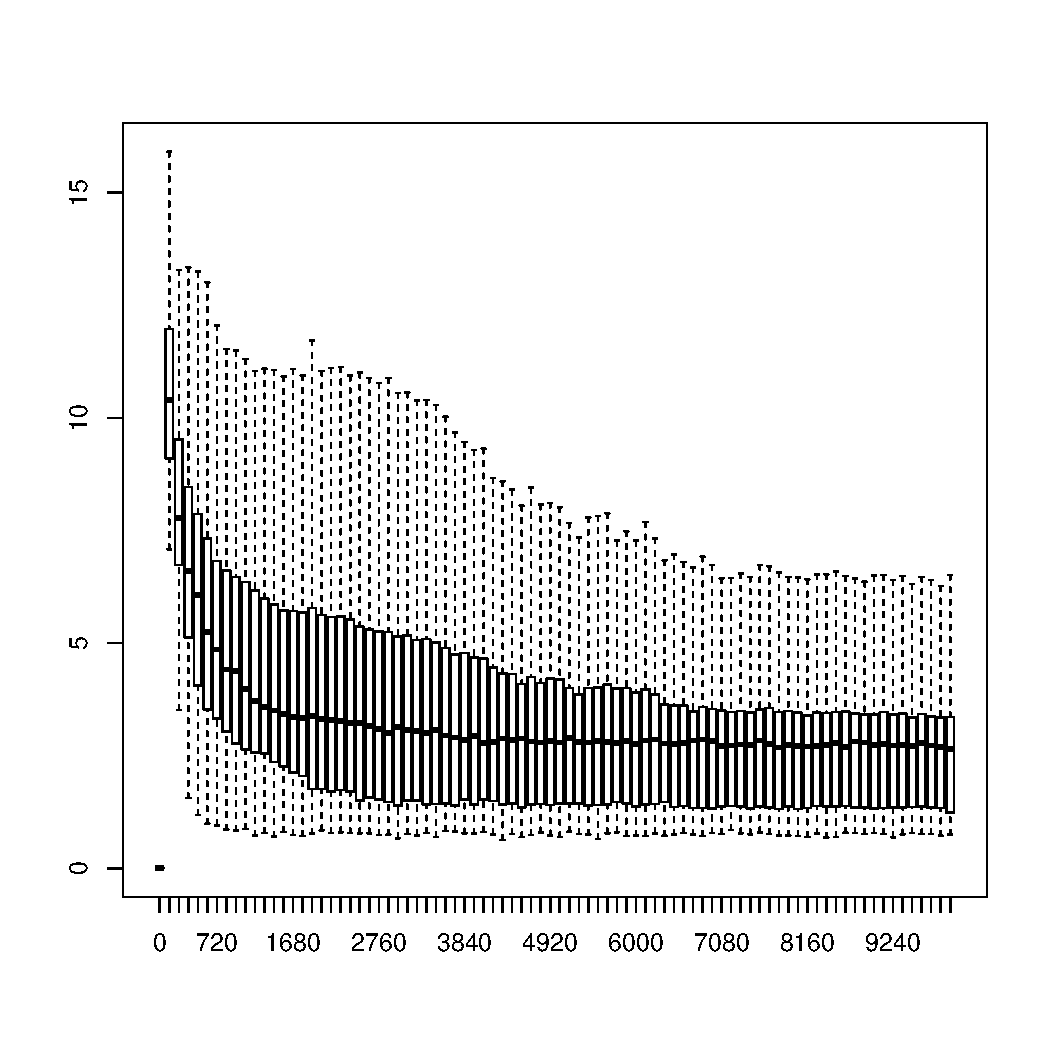
\includegraphics[width=5cm]{img/full.pdf} 
							\caption{Evolution of the score of the agents in a setup with 600 agents and 3 goods trading and exchanging their strategies during 10000 timesteps.}%%
							\label{fig:scoreEvol}
						\end{multicols}
					\end{figure}
					\vspace{-1cm}
					When the cultural network is fully connected, all the mean score of the agent converge to a value around 3. It means that during the 10 exchange they make, in the worst case there is 3 exchanges during which they are not able to exchange one of the goods.
					\subsection*{Influence of Average Distance ($L$) and Average Degree ($\left\langle k\right\rangle$)}
					\begin{multicols}{2}
						To test the influence of the topology of cultural networks we design several networks with the same average distance $L$ and different average degree $\left\langle k\right\rangle$. 
						
						To reach those value, we create ring lattices of $v$ neighbours and then we rewire other ring lattices with $v'<v$ until the former network's $L$ is achieved.  
						\columnbreak
						\begin{center}
							\Large
							\begin{tabular}{l|ccc}
								& $\left\langle k\right\rangle_1$	 	& \dots & $\left\langle k\right\rangle_n$		\\\hline
								$L_1$	& $G_{11}$	& 	& $G_{1n}$	\\	
								\dots	&		&\dots	&		\\
								$L_m$	& $G_{m1}$	& 	& $G_{mn}$	\\	
							\end{tabular}
						\end{center}
					\end{multicols}

					\columnbreak 

					The next table illustrates some of the topologies we designed for networks with 200 agents and for some couple of values $\{L,\left\langle k\right\rangle\}$.
					\begin{center}
						\begin{tabular}{m{1.2cm}m{2cm}m{2cm}}
							&$\left\langle k\right\rangle=0.02$ & $\left\langle k\right\rangle=0.04$\\
							$L\approx17$&
							
\includegraphics[width=2cm]{img/g02.pdf}&
							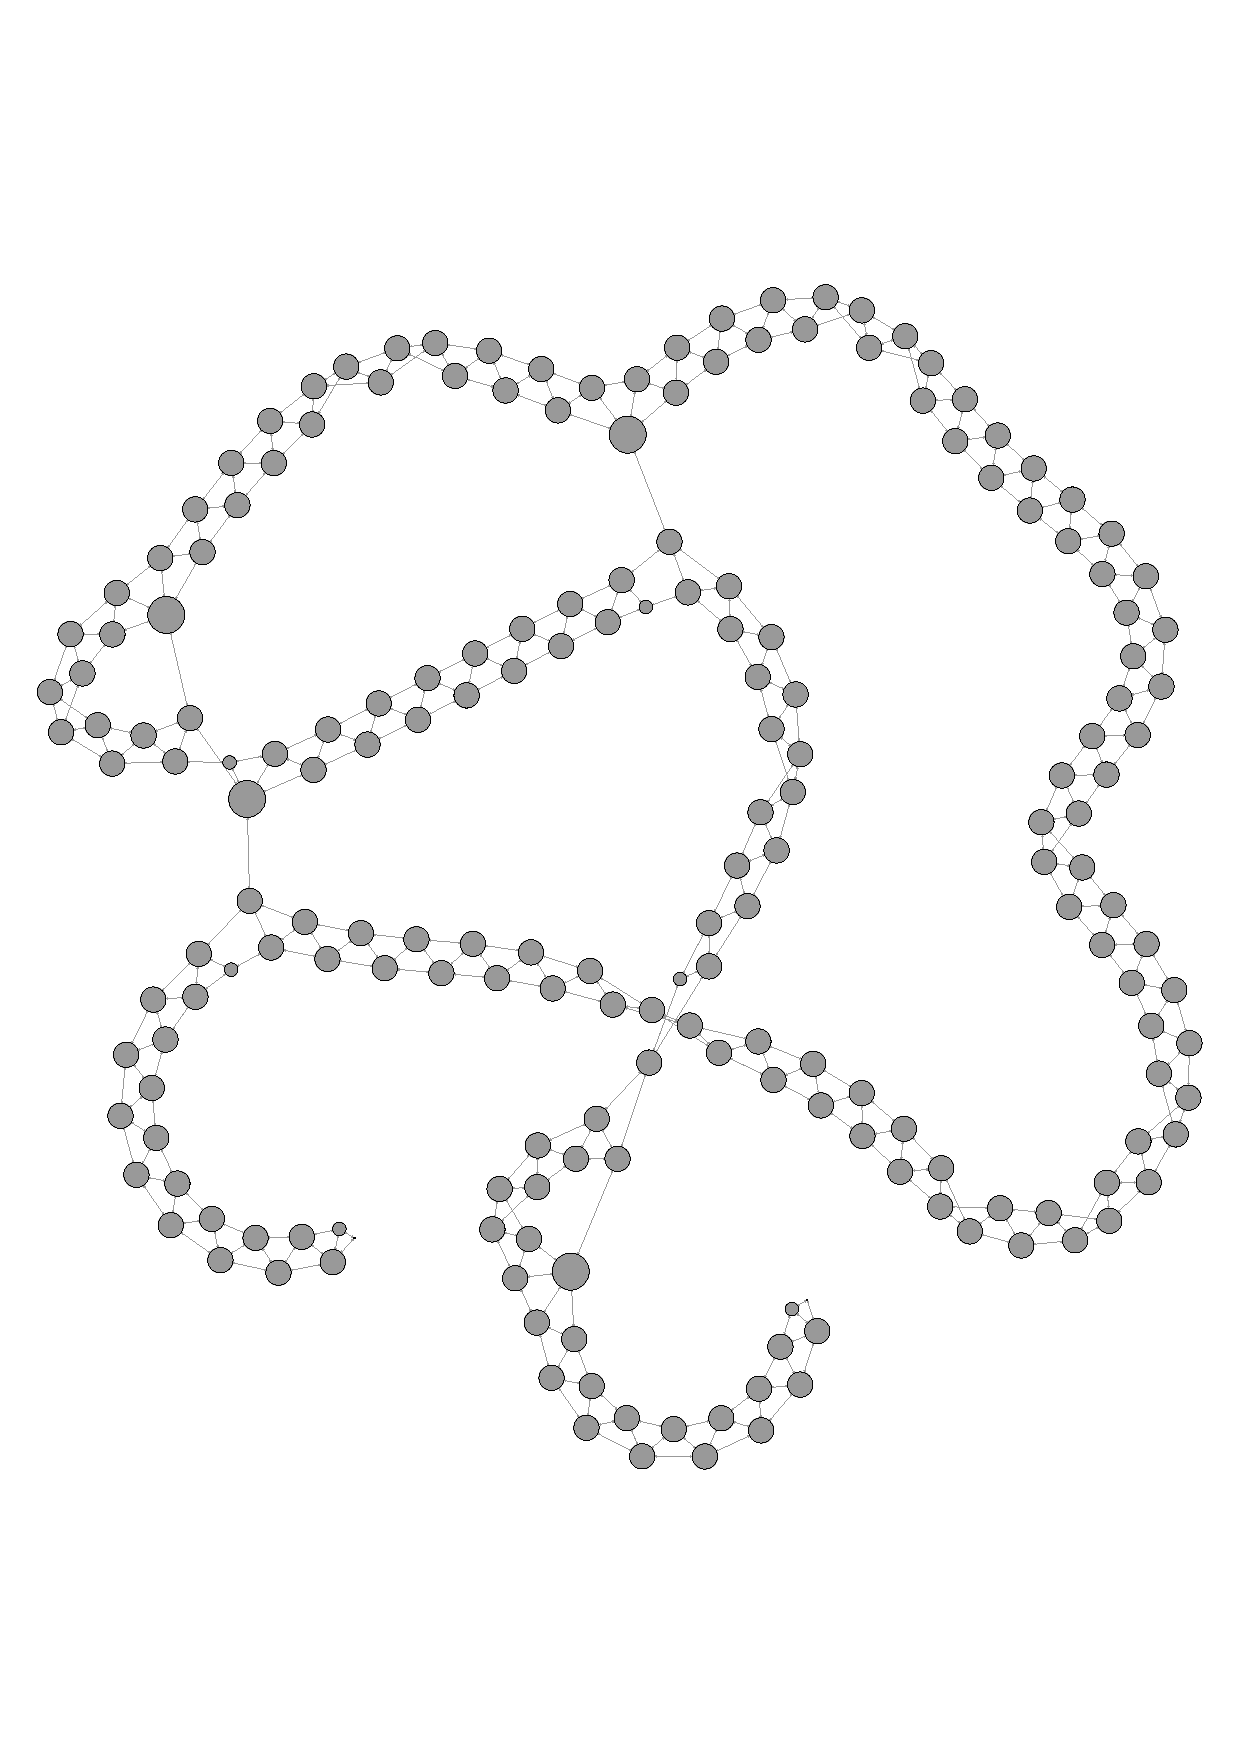
\includegraphics[width=2cm]{img/g00.pdf}\\
							$L\approx4$&
							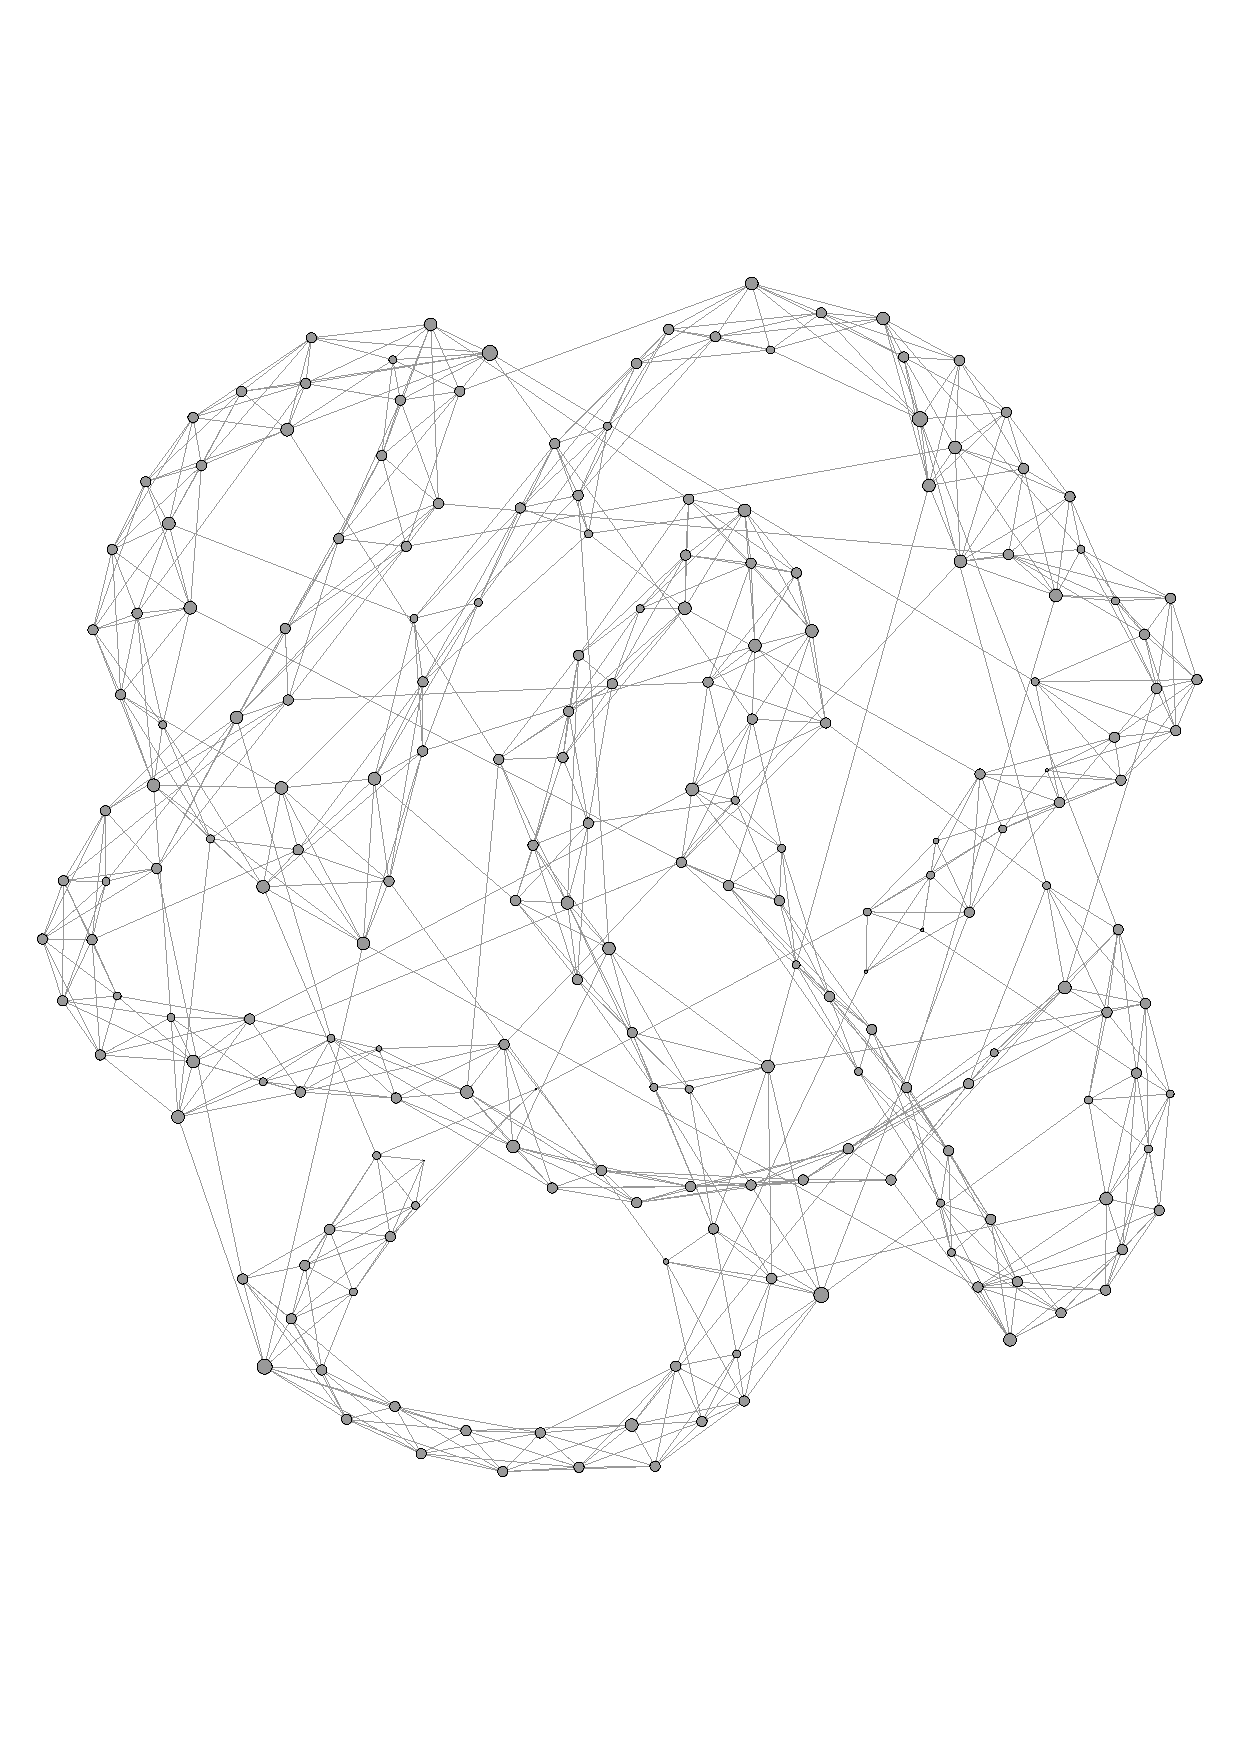
\includegraphics[width=2.5cm]{img/g42.pdf}&
							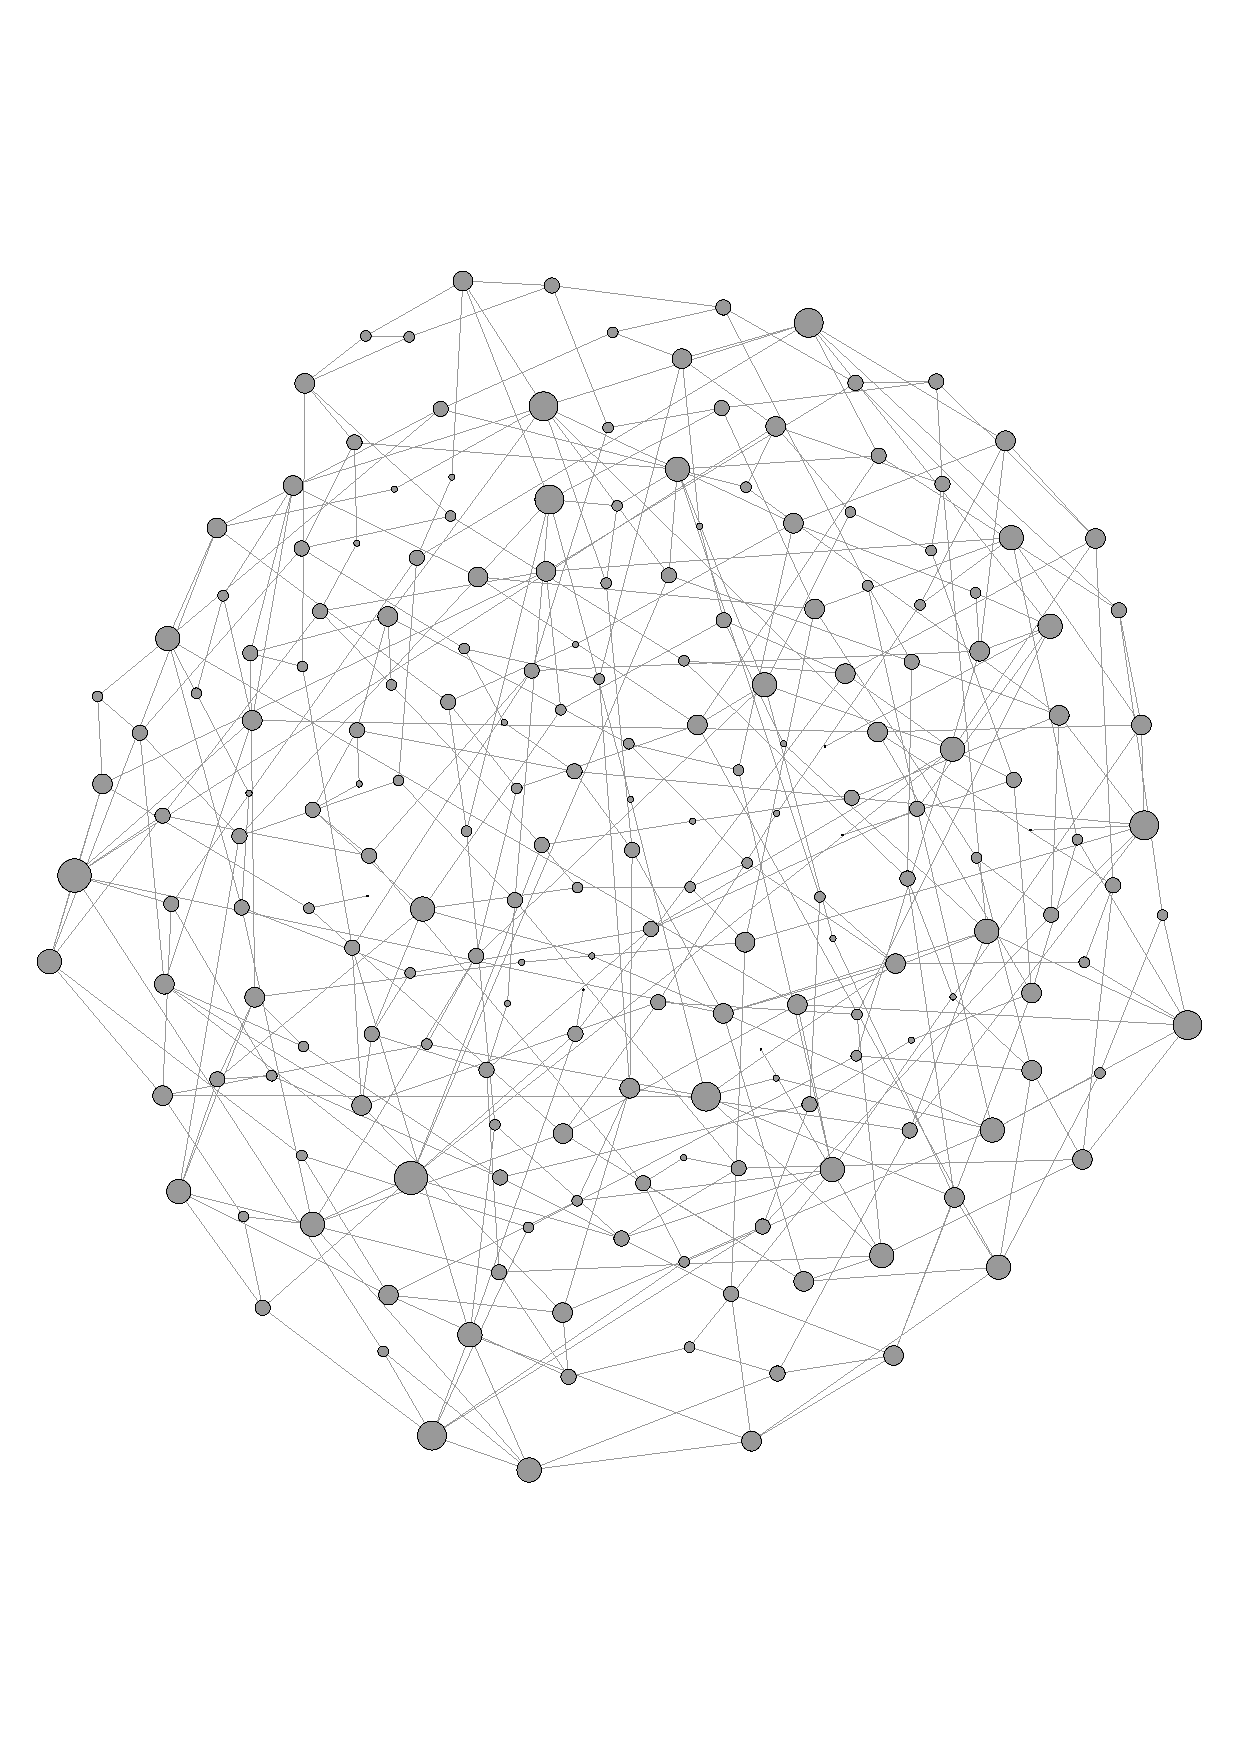
\includegraphics[width=2.5cm]{img/g40.pdf}\\
						\end{tabular}
					\end{center}
					\subsection*{Results}
		%As shown by the figure~\ref{fig:ratioEvol}, the raise of the score of the agents comes from the fact that the mechanism of $CulturalTransmission$ biased by the economic success of the agents allows them to quickly estimates prices that converge toward their optimal value . Thus it allows them to make more efficient trade and increase their economic success (see also \cite{gintis_emergence_2006}).
					The average distance $L$ have been proven to be the key property for the simulations not only to reach the equilibrium faster, but also to show better performances for the agents. For equal values of $L$. 
					\begin{figure}[H]
						\center
						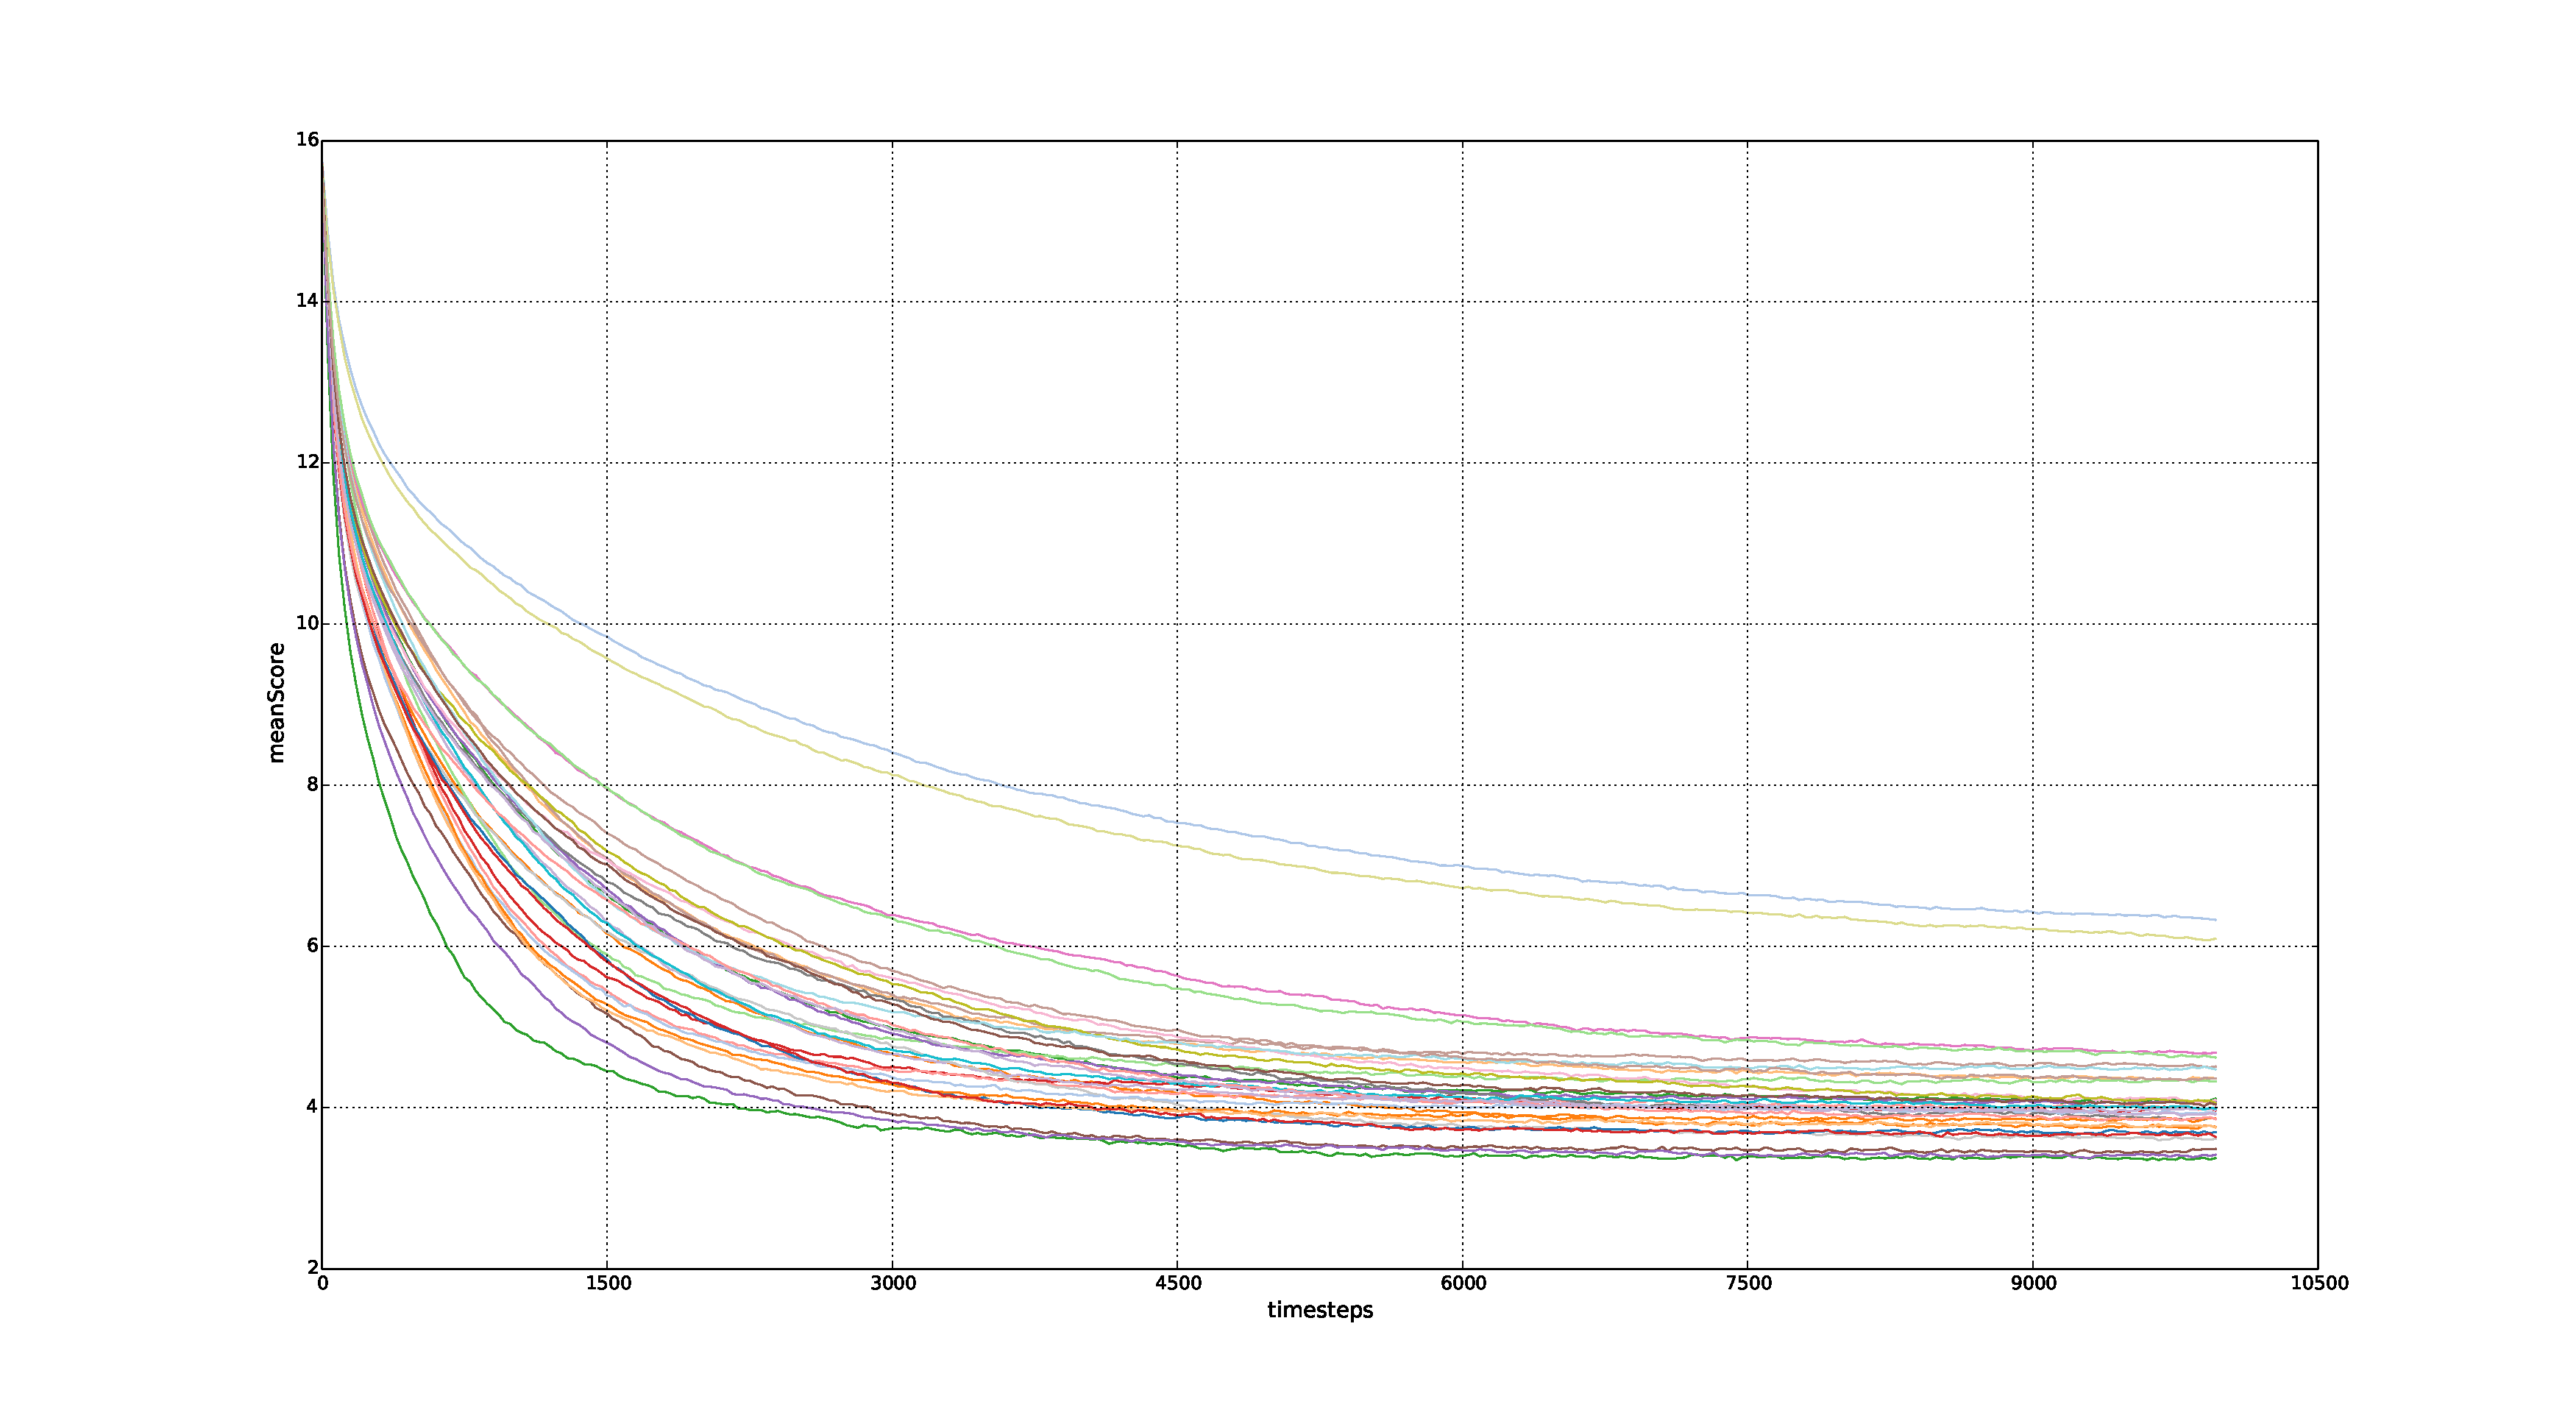
\includegraphics[width=5cm]{img/provResults2.pdf}
						\caption{ \small
						Behaviour of the simulations with different topologies.}
						\label{fig:results2}
					\end{figure}



				\end{multicols}
			}
			\headerbox{Concluding Remarks}{name=conclusion,column=0,below=res1}{
				Integrating cultural and economic dynamics into an evolutionary framework is a good candidate to study such systems. It allows one to study precise mechanisms and to easily test and compare different model of such mechanisms.

				In future works we hope to fruitfully apply that tool to validate, interpret and propose hypotheses about economics and cultural dynamics at work during the Roman Empire.
			}


			\headerbox{References}{name=references,column=1,below=res1}{
				\scriptsize
				\renewcommand{\refname}{\vspace{-0.5em}}
				\bibliographystyle{unsrt}
				\bibliography{biblio}
			}
			\headerbox{Acknowledgements}{name=acknowledgements,column=1,below=references}{
				\begin{multicols}{2}

				Funding for this work was provided by the ERC Advanced Grant EPNet (340828).
				\begin{center}
					
\includegraphics[width=2cm]{logos/bscLogo.jpg}
	%\raisebox{.35\height}{
\includegraphics[width=1cm]{logos/logoSimpast.png}}
					
\includegraphics[width=1.5cm]{logos/LOGO-ERC.jpg}
				\end{center}
				\end{multicols}{2}
			} 

		\end{poster}

		\end{document}

